\documentclass[11pt]{article}
\usepackage[utf8]{inputenc}
\usepackage[a4paper,left=1in,right=1in,bottom=0.8in,top=0.8in,headheight=60pt,headsep=0.5cm]{geometry}
\usepackage{enumitem}
\usepackage[dvipsnames]{xcolor}
\usepackage{graphicx}
\usepackage{tikz}
\usepackage{transparent}
\usepackage{tabularx}
\usepackage{booktabs}
\usepackage{parskip}
\usepackage[ngerman]{babel}
\usepackage{setspace}
\usepackage{makecell}
% https://tex.stackexchange.com/a/176780
% \usepackage{ltablex}
% https://tex.stackexchange.com/a/26483
% https://tex.stackexchange.com/a/376804
\usepackage{multicol}
\usepackage{pbox}

% \usepackage{blindtext}

% \usepackage{libertine}
% \usepackage{pdfpages}

% ====== FONTS ======
	\usepackage[defaultfam,tabular,lining]{montserrat} %% Option 'defaultfam'
	%% only if the base font of the document is to be sans serif
	% \usepackage[T1]{fontenc}
	% \usepackage[scale=0.95,ttdefault=false]{AnonymousPro}
	% \usepackage{textcomp}
	\renewcommand*\oldstylenums[1]{{\fontfamily{Montserrat-TOsF}\selectfont #1}}
	% http://www.tug.dk/FontCatalogue/
	\renewcommand*{\ttdefault}{cmvtt}

	\pdfmapfile{+RobotoMono.map}
	\font\rbtmn=rbtmmn8t
	\font\rbtmnemail=rbtmmn8t at 9pt
	\font\rbtmnlinks=rbtmmn8t at 8pt

% ====== /FONTS ======

% Fancy Header
% \pagenumbering{gobble}
	\usepackage{fancyhdr}
	\usepackage{lastpage}
	\pagestyle{fancy}
	\fancyhf{}
	\renewcommand{\headrulewidth}{0pt}
	% \renewcommand{\headrulewidth}{0.1pt}
	% \renewcommand{\headrule}{\vspace{-10pt} \hbox to\headwidth{\color{headercol}\leaders\hrule height \headrulewidth\hfill}}
	% \lhead{\color{headercol} Curriculum Vitae}
	% \rhead{\color{headercol} Sun Yudong}
	\cfoot{\ttfamily \thepage\space von \pageref{LastPage}}
	% https://www.overleaf.com/learn/latex/Page_numbering
	% https://tex.stackexchange.com/a/74354

\usepackage{hyperref}
\hypersetup{
	pdftitle={Yudong Sun -- Lebenslauf},
	pdfauthor={Yudong Sun},
	bookmarksnumbered=true,
	bookmarksopen=true,
	bookmarksopenlevel=2,
	pdfstartview=Fit,
	pdfpagemode=UseOutlines,
	colorlinks=true,
	linkcolor=black,
	filecolor=magenta,
	urlcolor=black
}
\urlstyle{same}

\usepackage{titlesec}

\makeatletter
	\renewcommand\thesection{\two@digits{\value{section}}}
\makeatother
% https://tex.stackexchange.com/a/101714

% \titlespacing{command}{left spacing}{before spacing}{after spacing}[right]
\titlespacing\section{0pt}{18pt plus 4pt minus 2pt}{10pt plus 2pt minus 2pt} %https://tex.stackexchange.com/a/53341/116525

\titleformat{\section} % {command}
  {\normalfont\bfseries\Large}{\textcolor{gray}{\normalfont \ttfamily / \thesection}}{1em}{}
  % {format}{label}{sep}{beforecode}{aftercode}
  % https://tex.stackexchange.com/a/36611

\definecolor{section_1}{HTML}{00729c}
\definecolor{section_2}{HTML}{729c0f}
\definecolor{section_3}{HTML}{ff6400}
\definecolor{section_4}{HTML}{9c007f}
\definecolor{section_5}{HTML}{9c0024}
\definecolor{text_link}{HTML}{006080}
\definecolor{code_back}{HTML}{dddddd}
\definecolor{badgeback}{HTML}{393D43}
\definecolor{subheader}{HTML}{af0029}
\definecolor{skiheader}{HTML}{0392aa}
\definecolor{subtitles}{HTML}{a9a9a9}
\definecolor{headercol}{HTML}{aaaaaa}
\definecolor{schtitles}{HTML}{777777}
\definecolor{dark_gray}{HTML}{555555}

% \newcommand{\monoSp}[1]{{\fontfamily{qcr}\selectfont#1}}
\newcommand{\monoSp}[1]{{\usefont{T1}{rbtm}{m}{n} #1}}
\newcommand{\urllinkout}[2]{\href{#1}{\textcolor{text_link}{\small \texttt{#2}}}}
\newcommand{\linkout}[2]{\href{#1}{\textcolor{text_link}{#2}}}
% \newcommand{\code}[1]{\colorbox{code_back}{\monoSp{#1}}}
\newcommand{\code}[1]{\monoSp{#1}}
\newcommand{\badge}[1]{\colorbox{badgeback}{\color{white} \monoSp{#1}}}
\newcommand{\nummer}[1]{\texttt{\large #1}}
\newcommand{\job}[1]{\textbf{#1}}
\newcommand{\country}[1]{\textcolor{Mahogany}{#1}}

% For summary
% \setcounter{section}{-1}

\begin{document}

% https://tex.stackexchange.com/a/386331
\begin{tikzpicture}[remember picture,overlay,shift={(current page.north east)}]
    \node[anchor=north east,xshift=1.6mm,yshift=1.5mm]{
\includegraphics{header-deutsch.eps}};
    \node[anchor=north east,xshift=-6.17mm,yshift=-5.16mm]{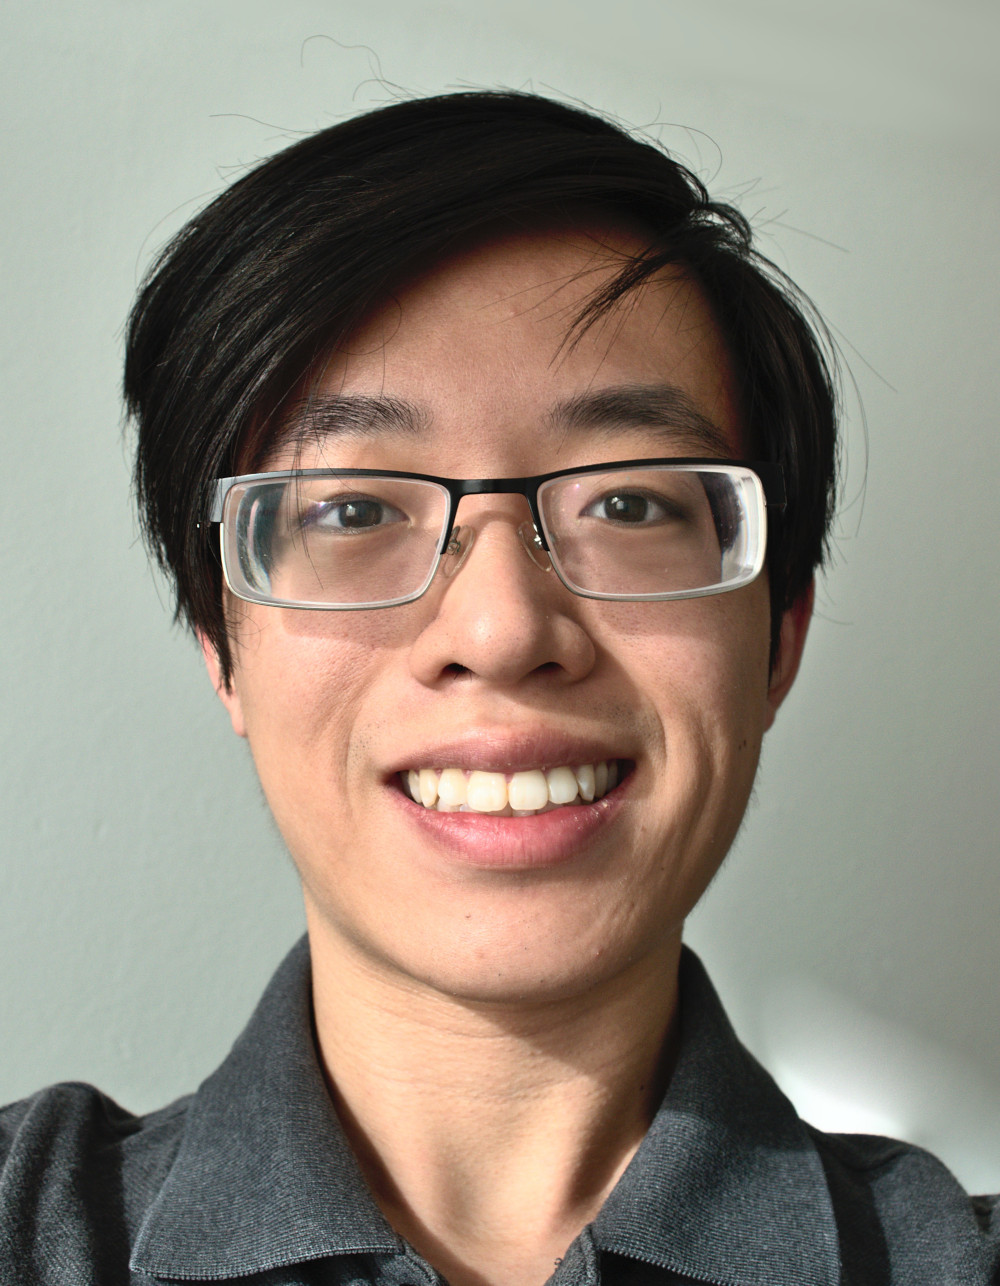
\includegraphics[width=32.78mm]{id.jpg}};
\end{tikzpicture}
\begin{tikzpicture}[remember picture, overlay]%
	\node[anchor=north west,yscale=2.3,xscale=2.13] at (-2.25, 2.08) {\textcolor{White}{\transparent{1}Yudong SUN}};%
    \node[] at (3.3, -0.45) {{\transparent{1}\fontsize{10}{10}{\rbtmnemail\href{mailto:Yudong.Sun@physik.uni-muenchen.de}{\textcolor{white}{Yudong.Sun@physik.uni-muenchen.de}}}}};%
    \node[anchor=north west] at (0.05, -0.655) {\textcolor{white}{\transparent{1}\fontsize{10}{10}{\rbtmnemail Waginger Straße 1}}};%
    \node[anchor=north west] at (0.05, -1.075) {\textcolor{white}{\transparent{1}\fontsize{10}{10}{\rbtmnemail 81549 München}}};%
    \node[anchor=north west] at (0.03, -1.585) {\textcolor{white}{\transparent{1}\fontsize{10}{10}{\rbtmnemail +49 162 5476221}}};%
    \node[anchor=north west] at (0.04, -2.050) {\textcolor{white}{\transparent{1}\fontsize{10}{10}{\rbtmnemail 1998-07-29}}};%
    % \node[] at (10.9, -2.3)  {{\fontsize{10}{10}\transparent{0}{\rbtmnlinks\href{https://github.com/sunjerry019}{github.com/sunjerry019}}}};% 14.8, -0.03, 14,65
    % \node[] at (10.45, -1.875) {{\fontsize{10}{10}\transparent{0}{\rbtmnlinks\href{https://linkedin.com/in/sunjerry019}{linkedin.com/in/sunjerry019}}}};%
\end{tikzpicture}
\vspace{2.8cm}

\fontsize{12}{13}\selectfont % https://tex.stackexchange.com/a/4140/116525

\section{\textcolor{section_1}{Bildung}}
	\begin{center}
		\renewcommand{\arraystretch}{1.3}
		\renewcommand{\cellalign}{lt}
		\begin{tabularx}{0.9\textwidth}{  p{4cm}  X  }
			\makecell{\texttt{\footnotesize seit} \\ \texttt{2019{\footnotesize /10}}} &
			\makecell{\textcolor{schtitles}{\small \textit{Universität}} \\ \job{Ludwig-Maximilians-Universität München}, DE\\Physik, B.Sc. \hfill 2. Semester} \\ % \vspace{0.5em}  [1.5em]
			\midrule
			\texttt{2016{\footnotesize /12}} & \makecell{\textcolor{schtitles}{\small Schulabschluss} \\\job{School Graduation Certification} \hfill \texttt{\small Note: 1,1}  \\ --- {\scriptsize Singapore-Cambridge GCE Advanced Level Examination} \vspace{0.5em}}\\
			\midrule			
			\makecell{\texttt{\footnotesize von} \hspace{2.4em} \texttt{\footnotesize bis} \\ \texttt{2015{\footnotesize /01}} - \texttt{2016{\footnotesize /12}}} & \makecell{\textcolor{schtitles}{\small \textit{Junior College {\footnotesize (voruniversitäre Bildung)}}} \\ \job{Hwa Chong Institution (College)}, SG 
				\\ --- {\scriptsize Hwa Chong Diploma with Distinction}
				\\ --- {\scriptsize \href{https://en.wikipedia.org/wiki/International_Science_Youth_Forum_@_Singapore}{International Science Youth Forum @ Singapore}}
				\\ {\transparent{0}---} \texttt{2016{\footnotesize /01}} {\scriptsize Organisator, Betreuer}
				\\ {\transparent{0}---} \texttt{2015{\footnotesize /01}} {\scriptsize Teilnehmer}
			} \\[1.5em]

			\makecell{\texttt{\footnotesize von} \hspace{2.4em} \texttt{\footnotesize bis} \\ \texttt{2011{\footnotesize /01}} - \texttt{2014{\footnotesize /12}}} & \makecell{\textcolor{schtitles}{\small \textit{Sekundarschule}} \\ \job{Hwa Chong Institution (High School)}, SG 
				\\--- \texttt{2014{\footnotesize /12}} {\scriptsize Schüler Austausch (\country{Xi'an, CN})}
				\\--- \texttt{2013{\footnotesize /12}} - \texttt{2014{\footnotesize /08}} {\scriptsize Schüler Austausch (\country{Virginia, US})}
				\\ {\transparent{0} --- ---}{\footnotesize Loudoun Academy of Science}
				\\ {\transparent{0} --- ---}{\footnotesize Gemeinsame Arbeit an eine Forshungsprojekt}
				\\ {\transparent{0} --- ---}-- {\scriptsize \textit{Thema: Bioremediation}}
				\\--- \texttt{2013{\footnotesize /06}} {\scriptsize Schüler Austausch (\country{Frankenberg, Hessen, DE})}
				\\--- \texttt{2012{\footnotesize /11}} {\scriptsize Schüler Austausch (\country{Suzhou, CN})}
			} \\
			
			\makecell{\texttt{\footnotesize von} \hspace{2.4em} \texttt{\footnotesize bis} \\ \texttt{2005{\footnotesize /01}} - \texttt{2010{\footnotesize /12}}} & \makecell{\textcolor{schtitles}{\small \textit{Grundschule}} \\ \job{Nan Hua Primary School}, SG} 
		\end{tabularx}
	\end{center}
\section{\textcolor{section_2}{Praktika und Arbeitstätigkeiten}}
	\begin{center}
			\renewcommand{\arraystretch}{1.3}
			\renewcommand{\cellalign}{lt}
			\begin{tabularx}{0.9\textwidth}{  p{4cm}  X  }
				\makecell{\texttt{\footnotesize von} \hspace{2.4em} \texttt{\footnotesize bis} \\ \texttt{2019{\footnotesize /02}} - \texttt{2019{\footnotesize /09}}} & \makecell{\job{Forschungspraktikant} \\ 
					{\small National University of Singapore, SG} \\ 
					{\scriptsize Nanomaterials Research Lab} 
					\\ {\scriptsize Dazu auch Betreuung von Schüler aus \country{China}, \country{Taiwan}, \country{Indien}, u.a.}
					\\ --- \texttt{2019{\footnotesize /07}} {\scriptsize Wissenschaft Sommercamp}
					\\ --- \texttt{2019{\footnotesize /06}} {\scriptsize Physik-Anreichungscamp} 
				} \\
				\makecell{\texttt{\footnotesize von} \hspace{2.4em} \texttt{\footnotesize bis} \\ \texttt{2017{\footnotesize /02}} - \texttt{2019{\footnotesize /02}}} & \makecell{\job{Militärdienst}\\{\small Streitkräfte Singapurs, SG}} \\
				\makecell{\texttt{\footnotesize von} \hspace{2.4em} \texttt{\footnotesize bis} \\ \texttt{2017{\footnotesize /01}} - \texttt{2017{\footnotesize /02}}} & \makecell{\job{Lehrpraktikant}\\{\small Queensway Secondary School, SG}}
			\end{tabularx}
		\end{center}
\section{\textcolor{section_3}{Besonderes soziales Engagement}}
	\begin{center}
		\renewcommand{\arraystretch}{1.3}
		\renewcommand{\cellalign}{lt}
		\begin{tabularx}{0.9\textwidth}{  p{4cm}  X  }
			\makecell{\texttt{\footnotesize von} \hspace{2.4em} \texttt{\footnotesize bis} \\ \texttt{2018{\footnotesize /02}} - \texttt{2019{\footnotesize /09}}} & \makecell{\job{(Freiwilliger) Trainer des Schulteams}\\ \textit{\small Singapore Junior Physics Olympiad}
			\\ {\small \textcolor{dark_gray}{\textit{Hwa Chong Institution}}} \\ --- {\footnotesize Durchführung von wöchentlichen Lehr- und Übungseinheiten} 
			}  \\
			\makecell{\texttt{\footnotesize von} \hspace{2.4em} \texttt{\footnotesize bis} \\ \texttt{2015{\footnotesize /02}} - \texttt{2016{\footnotesize /06}}} & \makecell{\job{Coding4Children} \\ {\small Gründungsmitglied, Freiwilliger} 
			\\ {\small \textcolor{dark_gray}{\textit{Ulu Pandan Gemeindezentrum}}} \\
			--- {\footnotesize Das Beibringen von Grundschulschülern aus sozial benach-}\\
			{\transparent{0} ---}{\footnotesize -teiligten Familien die Programmierung.} \\
			--- {\footnotesize Das Ziel war es, sie für Programmierung zu begeistern und} \\
			{\transparent{0} ---}{\footnotesize ihnen zu helfen, eine Lebenskompetenz zu erlernen, die für} \\
			{\transparent{0} ---}{\footnotesize ihren zukünftigen Beruf nützlich sein kann.}
			} \\
			\multicolumn{2}{l}{Community Service Mithilfe bei verschienden Projekten}
		\end{tabularx}
	\end{center}
\section{\textcolor{section_4}{Sprachkenntnisse}}
	\begin{center}
		\renewcommand{\arraystretch}{1.3}
		\renewcommand{\cellalign}{lt}
		\begin{tabularx}{0.9\textwidth}{p{3cm}p{3cm} X}
			% \toprule
			Englisch & Muttersprache & Fließend \\
			Chinesisch & Muttersprache & Fließend \\
			Deutsch & Fremdsprache & \makecell{Sehr Gut\\TestDaF (TDN 4/5/4/4)}
			% \bottomrule
		\end{tabularx}
	\end{center}
\section{\textcolor{section_5}{Andere Interessen bzw. Fähigkeiten}}
	\begin{itemize}
		\item Informatik --- Programmierung {\small (Software Entwicklung, Automatisierung, u.s.w.)}
		\item Linguistik
		\item Fotographie
	\end{itemize}

\section{\textcolor{section_1}{Stipendien}}
	\begin{center}
		\renewcommand{\arraystretch}{1.3}
		\renewcommand{\cellalign}{lt}
		\begin{tabularx}{0.9\textwidth}{  p{4cm}  X  }
			\makecell{\texttt{\footnotesize von} \hspace{2.4em} \texttt{\footnotesize bis} \\ \texttt{2015{\footnotesize /01}} - \texttt{2016{\footnotesize /12}}} & \makecell{\job{German Language Elective Scholarship}\\ {\small Ministry of Education (Singapore), SG}} \\
			\makecell{\texttt{\footnotesize von} \hspace{2.4em} \texttt{\footnotesize bis} \\ \texttt{2011{\footnotesize /01}} - \texttt{2016{\footnotesize /12}}} & \makecell{\job{Edusave Entrance Scholarship} \\ {\small Top 3\% der nationalen Kohorte} \\ {\small Ministry of Education (Singapore), SG}} \vspace{0.3em} %  for Independent Schools
		\end{tabularx}
	\end{center}



\end{document}
